\documentclass[12pt]{article}
\usepackage{geometry}
\geometry{left=1in,right=0.75in,top=1in,bottom=1in}

\newcommand{\Problem}{D}
\newcommand{\Team}{2018506}

\usepackage{newtxtext}
\usepackage{amsmath,amssymb,amsthm}
\usepackage{newtxmath}

\usepackage[pdftex]{graphicx}
\usepackage{xcolor}
\usepackage{fancyhdr}
\lhead{Team \Team}
\rhead{}
\cfoot{}

\newtheorem{theorem}{Theorem}
\newtheorem{corollary}[theorem]{Corollary}
\newtheorem{lemma}[theorem]{Lemma}
\newtheorem{definition}{Definition}

\usepackage{bm}
\usepackage{booktabs}
\usepackage{multirow}
\usepackage{float}
\usepackage{subfigure}
\newcommand{\upcite}[1]{\textsuperscript{\textsuperscript{\cite{#1}}}}

\begin{document}
\graphicspath{{.}}
\DeclareGraphicsExtensions{.pdf, .jpg, .tif, .png}
\thispagestyle{empty}
\vspace*{-16ex}
\centerline{\begin{tabular}{*3{c}}
        \parbox[t]{0.3\linewidth}{\begin{center}\textbf{Problem Chosen}\\ \Large \textcolor{red}{\Problem}\end{center}}
         & \parbox[t]{0.3\linewidth}{\begin{center}\textbf{2020\\ MCM/ICM\\ Summary Sheet}\end{center}}
         & \parbox[t]{0.3\linewidth}{\begin{center}\textbf{Team Control Number}\\ \Large \textcolor{red}{\Team}\end{center}} \\
        \hline
    \end{tabular}}
\begin{center}
    \Large{Looking into the Football Teamwork through the Pass Network}
\end{center}

The teamwork plays important role in completing difficult tasks in today's interconnected society. In a team, people form a complex network, which has massive nodes and links and varies with time. The study of teamwork in football matches may offers us keys to team success. Here, we propose a model to analyze the team process of football team, Huskies, in the 38 matches last season.

First, to depict the cooperation relationship in the team, we construct an unidirectional, weighted pass network from the record of the pass events between the players, where the nodes present the players and the links indicate the cooperation between the players. The link weight characterizes the contribution of the cooperation between certain player pairs to the success of a match, which is related to the three factors: the possessing of the ball, the quality of the pass and the effect after the pass. We introduce concepts such as ball possessing factor and threatening degree to quantify these three factors.

Then we identify the typical cooperation pattern by comparing the motif number in the pass network obtained above with it in randomly-generated networks. We found that all of the three types of cooperation pattern, dyadic, triadic and clustered, appear in Huskies during the matches, and the specific type of cooperation patterns differs for the different matches.

We use pass number and the link weight in the pass networks as two indicators of teamwork's success and find the correlation between the indicators and Huskies' score. We investigate the indicator in multiple dimensions and scales:
\begin{itemize}
	\item \textbf{Time dimension, long-term scale.} We find Huskies score increases with the total pass number and total link weight in a whole match.
	\item \textbf{Time dimension, short-term scale.} We study how the pass number and the link weight per minute varies, and find that the end of a match is the period with weakest team cooperation.
	\item \textbf{Spatial dimension.} We depict the distribution of the pass number and link weight on the football field, and find that Huskies tend to pass the ball to the left side of the field but the actually advantageous attacking strategy for Huskies is from the right.
	\item \textbf{Player dimension, micro scale.} We use the pass number and the weight of corresponding link of each nodes to evaluate the contribution of the individual players.
\end{itemize}

According to what we learn about the two indicators, we list the following suggestions for improving Huskies performance in matches:
\begin{itemize}
	\item More frequent, safer and smarter passes can keep the team in advantageous situation and help score.
	\item The best team combination is forward 2, 6, midfield 1, 2, 3, 7, defense 1, 3, 4, 9, and goalkeeper 1.
	\item Attack from the right side rather than left.
	\item Keep alert and serious at the end of each match.
	\item Increase stamina training.
\end{itemize}

Close cooperation relationships, good combination of teammates and correct work strategies are the key for Huskies' and maybe also other teams' success. The methodology of constructing and analyzing the network of a team may also work for researches on the team process in other field.

\clearpage
\pagestyle{fancy}
\tableofcontents
\newpage
\setcounter{page}{1}
\rhead{Page \thepage\ }

\section{Introduction}
\subsection{Background}
Teamwork proves to be an effective method to complete complex tasks unattainable through either individual effort or simple sequential addition of teammates' contribution. However, the mechanism for making a successful team work is quite complicated. This is because, in teamwork, the cooperation between teammates forms intricate networks with massive nodes and links varying with time. Studying of the team process in football matches may offer valuable insight into the rules for teamwork's success in other field.

Actually, the previous work on the team process in football matches has been for over half century. As early as 1950s, Charles Reep began studying the hand-collected football match statistics and concluded that "the key to scoring goals is to transfer the ball as quickly as possible from back to front"\upcite{reep1968skill}. Later, the newly developed sensing technology offered researchers data with higher fidelity and the advance of network science opened a new perspective on football match analysis. In late seventies, Gould and Gatrell\upcite{gould1979structural} first introduced the concept of passing network among the football players but did not get enough attention. After thirty years, the seminal work by Duch and collaborators\upcite{duch2010quantifying} started the trend of analysis of football team with network science methodology.

% However, the present research on performance of the football team in matches remains on some specific scale. Some researchers like Buldú only focus on the average characterization of all the players in a team, others pay too much attention on the evaluation of individual's performance. Also, 

\subsection{Our Work}
Through analyzing Huskies' match data from last season, we propose an over-all models for studying the rules of teamwork's success. Our work consists of mainly five steps:
\begin{itemize}
    \item Create football passing networks in matches with players as nodes and the passing events as links between the nodes.
    \item Identify the network motif by comparing our passing network with a randomly generated network with the same numbers of nodes and links.
    \item Explore the indicators for Huskies' success in matches.
    \item Analyze the dynamic evolution of the success indicators.
    \item Give suggestions for improving team performance in both football matches and other fields.
\end{itemize}

% \subsection{Terminologies Explanation}
% Here are some terminologies that we will use in the following sections:

\subsection{Notation Description}
Here are the definitions of the main variables used in our modeling:
\begin{table}[h]
    \centering
    \caption{Main Variables}
    \label{Variables}
    \begin{tabular}{cp{12cm}}
        \toprule
        Symbols           & Definitions \\
		\midrule
		$x,y$ & The $x$- and $y$-coordinate on the football field, the range of which are both $[0,100]$. $x=0$ represent the goal of the attacking team and $x=100$ represent the goal of the other team. $y=0$ represents the attacking team's left-hand side, and $y=100$ represent the team's right-hand side.\\
		$W_{m,n}$               & The weight of the network link directed from player $m$ to player $n$. \\
		$w_{m,n,k}$ & The contribution to $W_{m,n}$ due to the $k$th pass from player $m$ to player $n$. \\
		$B$ & The basic contribution to link weight due to each pass. \\
		$E_{m,n,k}$ & The contribution to link weight due to the effect of the pass on the next event. \\
		$S_{m,n,k}$ & The extra contribution to link weight due to shot following the pass.\\
        \bottomrule
    \end{tabular}
\end{table}

\newpage

Some trivial variables will be described at the proper places of the following.



\subsection{Assumptions and Justification}
Here are some assumptions and justifications needed in our modeling:
\begin{itemize}
	\item The performance of Huskies is mainly related to some properties in their teamwork, but not the opponents'. (We will verify this later.)
	\item For simplicity, we do not take the events other than pass, duel and shot into consideration.
\end{itemize}

A few assumptions will be added at the proper place of the following article.

\subsection{Setting of the Matches}
According to the standard set by The International Football Association Board (The IFAB) for World Cup, the football field is a rectangle, with length of $105$ meters and width of $68$ meters. Two goal, with width of $7.32$ meters, are located at the midpoint of two short edges of the field, respectively. More detailed configuration of the football field is shown in figure \ref{The football field configuration}. A football match is divided into two 45-minute periods and involves two team both with 11 players, one of which is the goalkeeper, respectively. Other types of player are forward, defense, midfield. The aim of each team is to shot the ball into the opponent's goal while preventing the opponent's score.
\begin{figure}[h]
	\centering
	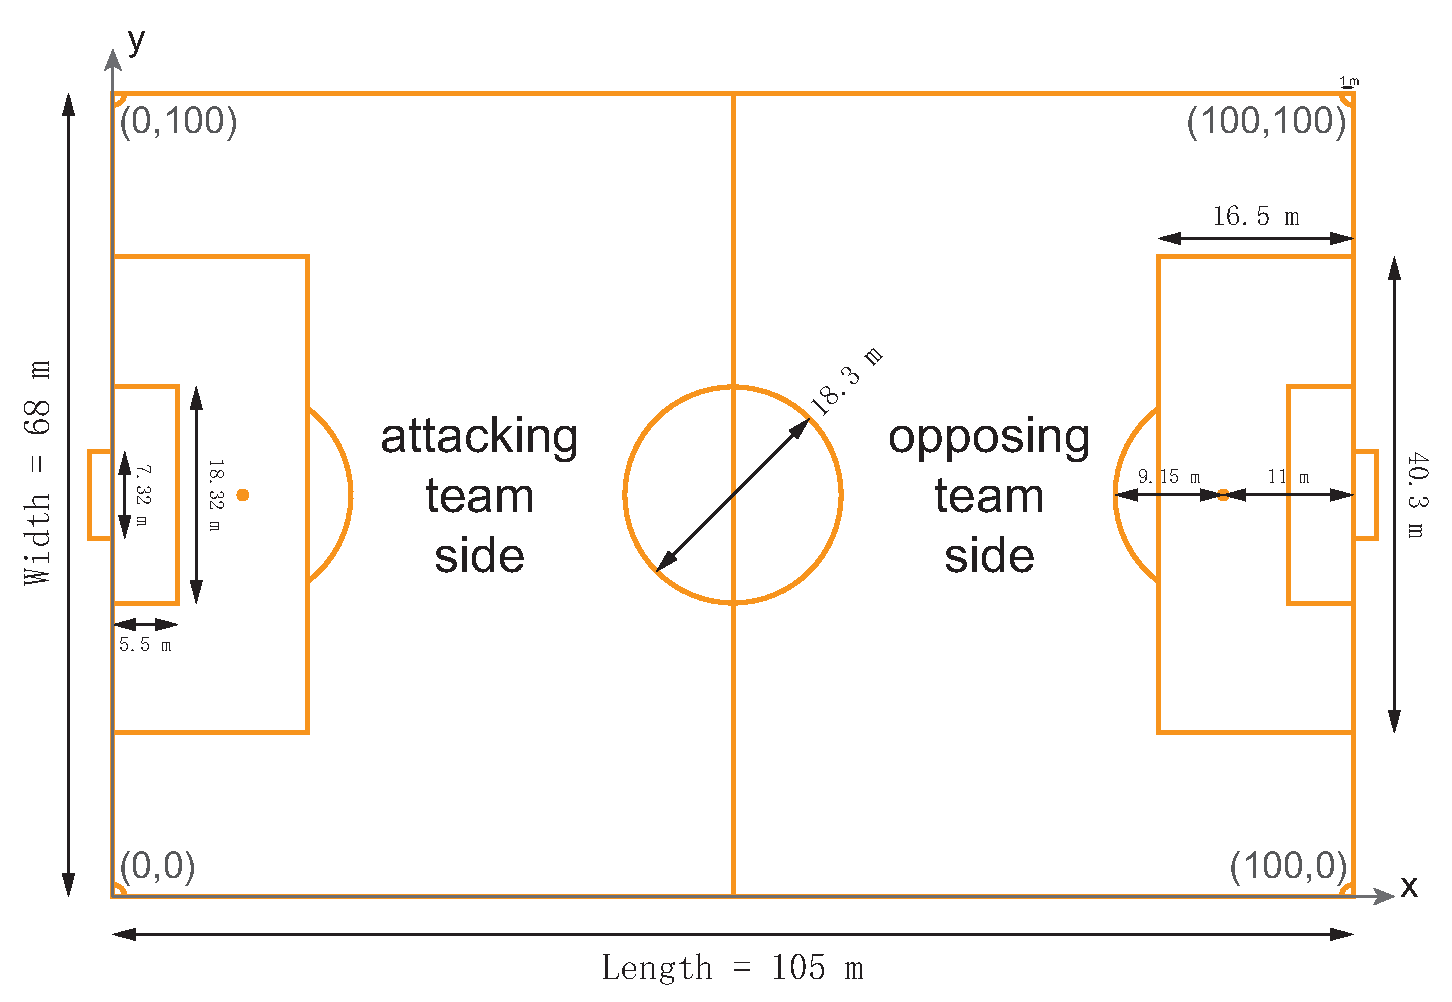
\includegraphics[width=.8\textwidth]{FootballField.eps}
	\caption{The football field configuration.}
	\label{The football field configuration}
\end{figure}

\section{The Pass Network}

\subsection{Construction of the Pass Network}

We construct the football pass network from the record of the ball passing events between the players. In the pass network, the nodes represent the football players and the edges, which is unidirectional and weighted, account for the ball passing between the players. The positions where the nodes placed is the average origin positions from which the players pass the ball:
\begin{gather}
	\label{meanx}\langle x_n\rangle=\frac{1}{K_n}\sum_{k=1}^{K_n}x_{n,k}\\
	\label{meany}\langle y_n\rangle=\frac{1}{K_n}\sum_{k=1}^{K_n}y_{n,k}
\end{gather}
where
\begin{itemize}
	\item[] $K_n$ is the total pass times of player $n$,
	\item[] $x_{n,k}$ is the $x$-coordinate of player $n$ when he passes the ball for the $k$th time,
	\item[] $y_{n,k}$ is the $y$-coordinate of player $n$ when he passes the ball for the $k$th time.
\end{itemize}

The weight of the links characterizes the importance of the cooperation between the player pairs, and every pass has contribution to the weight of the link corresponding to the origin and destination player:
\begin{equation}
	\label{linkweight}W_{m,n}=\sum_{k=1}^{K_n}w_{m,n,k}
\end{equation}
where
\begin{itemize}
	\item[] $W_{m,n}$ is the weight of the link from player $m$ to player $n$,
	\item[] $w_{m,n,k}$ is the contribution of the $k$th pass from player $m$ to player $n$.
\end{itemize}
We propose that the contribution of each pass consists of three part:
\begin{equation}
	w_{m,n,k}=B+E_{m,n,k}+S_{m,n,k},
\end{equation}
where:
\begin{itemize}
    \item \textbf{$B$ is the basic contribution due to possessing the ball.} Since the players at the origin and the destination of a pass are both Huskies, the pass means Huskies' possessing the ball for the short period during the pass, which adds to the safety and initiative to Huskies. In this way, every pass should have a basic contribution to the weight of the link. We set this basic contribution to be a constant:
    \begin{equation}
        B=0.1.
    \end{equation}
	\item \textbf{$E$ is the contribution due to the effect on the subsequent match.} Every pass updates the ball's position and thus have effect on the subsequent process of the match, which may have a positive or negative contribution to the link weight. This kind of contribution is related to two factors.
	\begin{itemize}
		\item First, the effect of a pass to the next event is concerned with its origin and destination position. To quantify how advantageous the pass's origin and destination position are for Huskies, we introduce the \textit{threatening degree}, which is a function of the ball's coordinate. Just as its name implies, the threatening degree of Huskies to the opponent team quantifies to what extent Huskies threatens the opponent team when Huskies possesses the ball. As shown in figure \ref{The player-goal triangle}, a Huskies player with the ball and the opponent's goal (regarded as a line segment in the 2D diagram) forms a triangle. $c$ is the width of the opponent goal and $a$, $b$ are the length of the other two edges of the triangle. $d$ is distance between the opponent goal midpoint and the player with the ball and $\theta$ is the opening angle of the goal to the player. Obviously, shorter $d$ and wider $\theta$ increase the possibility that Huskies shots and score, so we define the threatening degree as
		\begin{equation}
			T_h(x,y)=\frac{1}{2}T_h^{(d)}+\frac{1}{2}T_h^{(\theta)},
		\end{equation}
		where
		\begin{itemize}
			\item[] $T_h^{(d)}$ is the function of $d$. The smaller $d$ is, the greater $T_h^{(d)}$ is.
			\item[] $T_h^{(\theta)}$ is the function of $\theta$. The greater $\theta$ is, the greater $T_h^{(\theta)}$ is.
		\end{itemize}
		\begin{figure}[h]
			\centering
			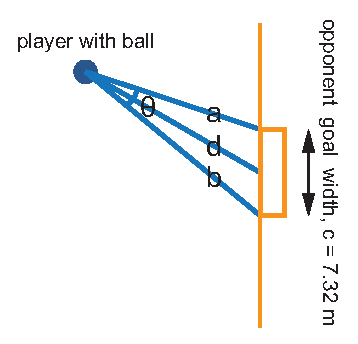
\includegraphics[scale=1]{FootballField2.eps}
			\caption{The player-goal triangle.}
			\label{The player-goal triangle}
		\end{figure}
		For convenience of calculation, we express the distance $d$ with the player's coordinate $x$ and $y$:
    	\begin{equation}
        d=\sqrt{\left[\frac{105}{100}(100-x)\right]^2+\left[\frac{68}{100}(y-50)\right]^2}.
		\end{equation}
		Since $0\leq x\leq 100$ and $0\leq y\leq 100$, the range of the distance is
   		\begin{equation}
    		0\leq d\leq 110.
		\end{equation}
		We normalize the range of $T_h^{(d)}$ to $[0,1]$ by defining
	    \begin{equation}
    	    T_h^{(d)}=\left(1-\frac{d}{110}\right)^2.
		\end{equation}
		As for the angle part, we express the opening angle $\theta$ as
		\begin{equation}
			\theta(x,y)=\arccos\frac{a^2+b^2-w^2}{2ab},
		\end{equation}
		where the two edges of the player-goal triangle satisfy
		\begin{gather}
        	a^2=\left[\frac{105}{100}(100-x)\right]^2+\left[\frac{68}{100}(y-50)-\frac{7.32}{2}\right]^2,\\
        	b^2=\left[\frac{105}{100}(100-x)\right]^2+\left[\frac{68}{100}(y-50)+\frac{7.32}{2}\right]^2.
		\end{gather}
		Considering that the range of $\theta$ is $[0,\pi]$, we normalize $T_h^{(\theta)}$ by defining
		\begin{equation}
			T_h^{(\theta)}(\theta)=\frac{\lg(\theta+1)}{\lg(\pi+1)}.
		\end{equation}
		Therefore, the threatening degree of Huskies to the opponent is
		\begin{equation}
			T_h=\left(1-\frac{d}{100}\right)^2+\frac{\lg(\theta)}{\lg(\pi+1)}.
		\end{equation}
		The distribution of the threatening degree of Huskies to the opponent is shown in figure \ref{FootballFieldWithThreateningDegree}. Similarly, we can also calculate the threatening degree of the opponent team to Huskies, denoted as $T_o$. We omit the specific formula of $T_o$ for concision.
		\begin{figure}[h]
			\centering
			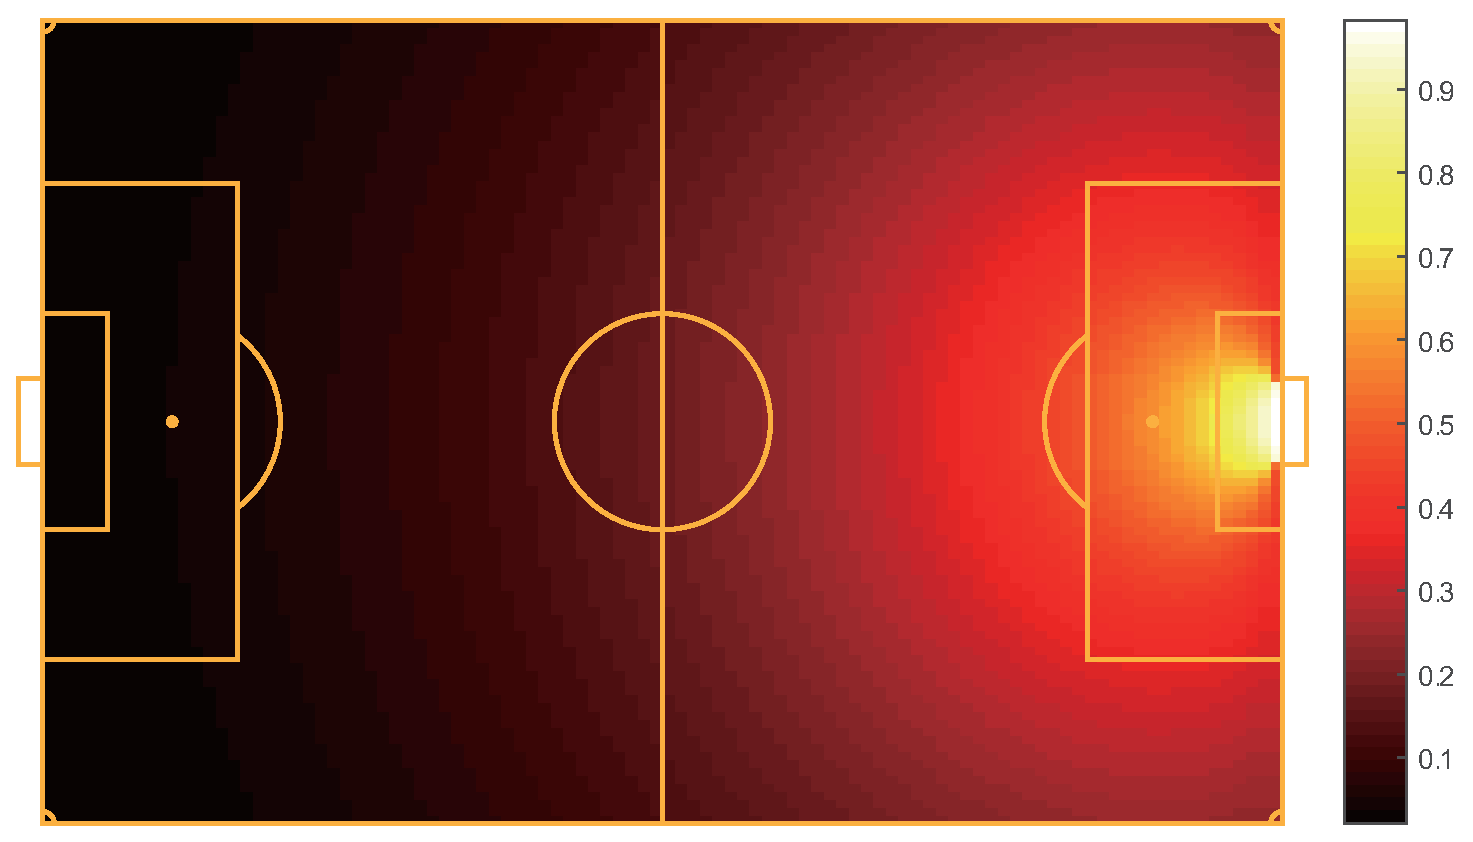
\includegraphics[width=.8\textwidth]{FootballFieldWithThreateningDegree.eps}
			\caption{Threatening degree distribution on the football field.}
			\label{FootballFieldWithThreateningDegree}
		\end{figure}
		\item The effect of a pass is also reflected on the next event happens after the pass. Regarding the type of next event, we divide the pass events into four categories: good pass, safe pass, dangerous pass and bad pass, as show in table \ref{Catagories of passing events}. The good pass is followed by a shot by the same team. The shot next to the pass implies that the pass creates a good opportunity for another player to launch an attack. The pass followed by another pass of the same team is classed as a safe pass since the ball is still in the control of the same team. If the ball falls into the duel of two teams after the pass, the pass is a dangerous pass. As for a bad pass, it result in the change hands of the ball in the next event.
		\begin{table}[h]
			\caption{Catagories of pass events.}
			\label{Catagories of passing events}
			\begin{tabular}{cp{5cm}cccc}
			\toprule
			\multirow{3}{*}{Passing event categories} & \multirow{3}{*}{The type of the next event} & \multicolumn{4}{c}{Ball possessing factor}                               \\ \cline{3-6} 
													  &                                             & \multicolumn{2}{c}{Before the pass} & \multicolumn{2}{c}{Ater the pass} \\ \cline{3-6} 
													  &                                             & $p_{h,1}$             & $p_{o,1}$           & $p_{h,2}$            & $p_{o,2}$           \\ \midrule
			Good pass                                 & Huskies' shot                               & 1                 & 0               & 1                & 0               \\
			Safe pass                                 & Huskies' pass                               & 1                 & 0               & 1                & 0               \\
			Dangerous pass                            & Duel                                        & 1                 & 0               & 0.5              & 0.5             \\
			Bad pass                                  & Opponent team's pass, free kick or shot     & 1                 & 0               & 0                & 1              \\ \bottomrule
			\end{tabular}
		\end{table}
		\\For different events, the team possessing the ball is different, so we define the ball possessing factors, $p_h$ and $p_o$, where the subscript $h$ and $o$ represent Huskies and the opponent team, respectively. The ball possessing factor is a number that can be one of $\{0,0.5,1\}$, regarding the type of the event. During a pass event where Huskies players involve, the ball possessing factor is $p_h=1$ and $p_0$, which means Huskies possessing the ball during the pass event while the opponent team does not possess the ball. The ball possessing factors may change in the event after the pass. If the pass is a good pass or safe pass, Huskies will still dominate the ball, so $p_h=1$ and $p_o=0$ after the pass. If the pass is a bad pass, the opponent team deprives the control of the ball from Huskies, so $p_h=0$ and $p_o=1$ after the pass. If the pass is a dangerous pass, the ball fall into the duel of the two teams in other words, then $p_h=p_o=0.5$ after the pass. The change of the ball possessing factors for different pass events are also listed in table \ref{Catagories of passing events}.
		\end{itemize}
		Since only the threatening degree of the team possessing the ball has effective threatening to the other team, we introduce the \textit{net threatening degree}, which is the difference of the products of two teams' the ball possessing factor and the threatening degree. The net threatening degree of Huskies to the opponent team before a pass is
		\[
			p_{h1,k}T_{h1,k}-p_{o1,k}T_{o1,k},
		\]
		and the net threatening degree after the pass is
		\[
			p_{h2,k}T_{h2,k}-p_{o2,k}T_{o2,k},
		\]
		where the subscript $h$ and $o$ represent Huskies and the opponent team, the subscript $1$ and $2$ represent before and after the pass , and the subscript $k$ represents the $k$th pass, as mentioned before. We can formulate $E_k$ as the change of the net threatening degree before and after the pass:
		\begin{align}
			\nonumber E_k=&(p_{h2,k}T_{h2,k}-p_{o2,k}T_{o2,k})-(p_{h1,k}T_{h1,k}-p_{o1,k}T_{o1,k})\\
			=&\left\{\begin{array}{ll}
					T_{h2,k}-T_{h1,k},&\text{if the $k$th pass is a good or safe pass,}\\
					0.5T_{h2,k}-0.5T_{o2,k}-T_{h1,k},&\text{if the $k$th pass is a dangerous pass,}\\
					-T_{o2,k}-T_{h1,k},&\text{if the $k$th pass is a bad pass.}
				\end{array}\right.
		\end{align}
		\item \textbf{$S_k$ is the bonus contribution of good pass.} If the pass is a good pass, which means the pass offers convenience for later shot, the pass should have more contribution to the weight than other types of pass. We set this extra contribution to be a constant for good passes and zero for passes of other types:
		\begin{equation}
			S_k=\left\{\begin{array}{ll}
				0.3,&\text{if the $k$th pass is a good pass},\\
				0,&\text{otherwise.}
			\end{array}\right.
		\end{equation}
	\end{itemize}
Using equation (\ref{meanx}), (\ref{meany}) and (\ref{linkweight}), we can determine the position of the nodes and the width (proportional to the weight) between the nodes and thus depict the network of every team in every matches. A typical network, plotted according to the data of Huskies in match 9 is shown in figure \ref{Network13Huskies}.
\begin{figure}[h]
	\centering
	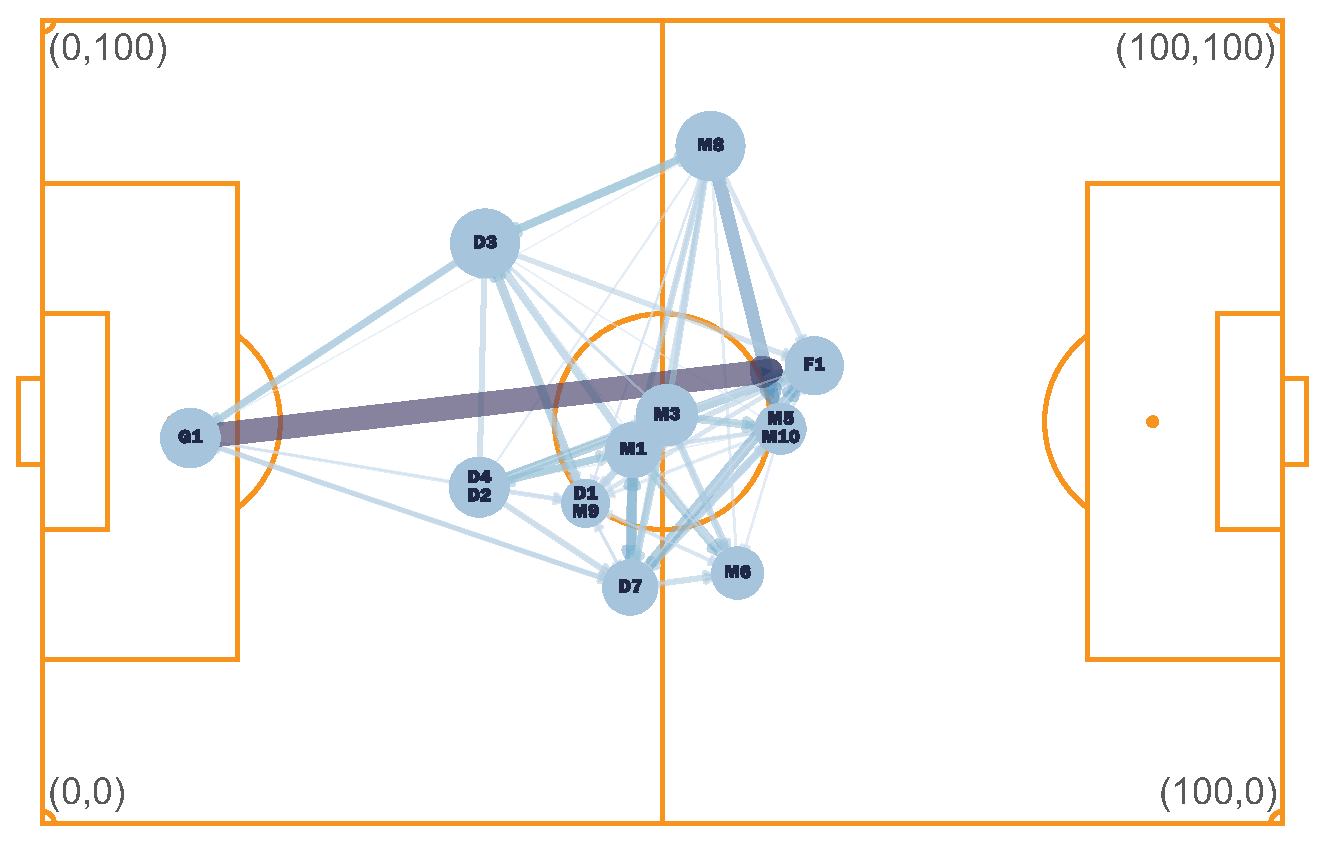
\includegraphics[width=.8\textwidth]{Network13Huskies.eps}
	\caption{The pass network of Huskies in match 13.}
	\label{Network13Huskies}
\end{figure}

\subsection{Identification of the Motifs in the Networks}
Motifs of network is some specific subgraphs appearing in the network much more frequently than in randomly generated networks\upcite{itzkovitz2005subgraphs}. The motifs of the pass networks we obtained above may tell us the typical cooperation patterns among the players in a match. The motifs can be divided into different types according to the number of nodes in the subgraph. For unidirectional networks like the pass network we obtained above, there may only be $2$ types of the $2$-node motifs (figure \ref{2nodemotifs}), $13$ types of 3-node motifs (table \ref{3nodemotifs}), and $9364$ types of $4$-node motifs\upcite{gursakal2018network}. Considering the instantaneity of football match process, we do not discuss the motifs with 4-nodes or higher numbers of nodes, since the time needed for the passes among $4$ or more players is so long that it can not be regarded as effective cooperation.

\textbf{$2$-node motifs}: The numbers of links in the pass networks of almost all the matches are over one hundred and very close to the total number of the links possible for a $11$-node network, $\frac{11!}{(11-2)!}=110$, which means almost all the possible links between the nodes exit in the pass network. (This fact can also be seen by eyes in the typical network shown in figure \ref{Network13Huskies}) In this way, we deduct that the $2$-node motif of the pass networks should be the type 2 in the figure \ref{2nodemotifs}.
\begin{figure}[h]
	\centering
	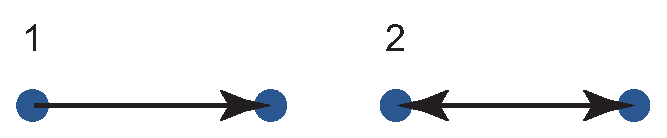
\includegraphics[width=.4\textwidth]{2NodeMotifs.eps}
	\caption{The two types of $2$-node motif.}
	\label{2nodemotifs}
\end{figure}

\textbf{$3$-node motifs}: Identification of the $3$-node motifs should be a little more difficult than that of $2$-node motifs. The identification algorithm is like this\upcite{gursakal2018network}:
\begin{itemize}
	\item Set the $20\%$ of the maximal link weight in the pass network as a filter threshold and filter out the links whose weight is below the threshold.
	\item Use the left links to construct a unweighted network and count the numbers of the $13$ types of $3$-node subgraphs. The number of the $i$th type of subgraphs is $N_{\text{pass},i}$.
	\item Randomly generate a set of networks which have the same in-degree and out-degree as the pass network, and count the numbers of $13$ types of $3$-node subgraphs. The average number of $i$th type of subgraphs is $N_{\text{rand},i}$ and the standard deviation is $\sigma_{rand,i}$.
	\item Calculate the $Z$ score of each subgraph:
	\begin{equation}
		Z_i=\frac{N_{\text{real},i}-N_{\text{rand},i}}{\sigma_{\text{rand},i}}.
	\end{equation}
	\item Compare the $Z$ scores of the subgraphs.
\end{itemize}
The $Z$ score indicate the typicality of a subgraph, so the subgraph with highest $Z$ score is the motif of the network, or, the most typical cooperation pattern among three players.

We calculate the $3$-node motifs of the pass network in $38$ matches and find the motifs of different matches are usually different. For example, the motif of match $16$ is the type 12, while the motif of match $25$ is type 7 as shown in table \ref{3nodemotifs}. We try to but can not related the motifs with the scores in these matches. Therefore, the typical cooperation varies with matches but do not have direct relation with the match outcome.
\begin{table}[h]
	\centering
	\caption{The $3$-node motifs.}
	\label{3nodemotifs}
	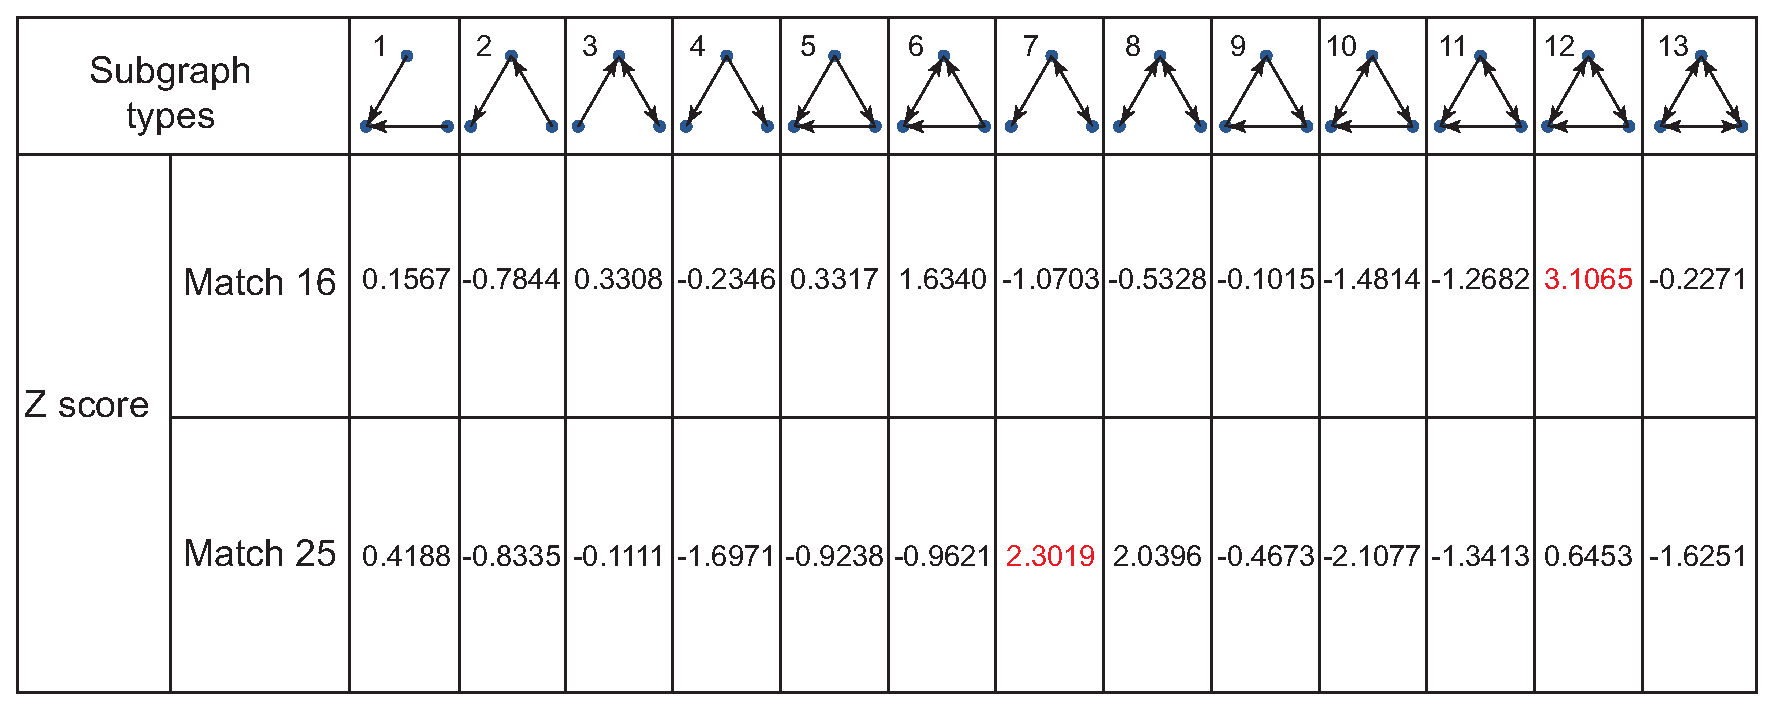
\includegraphics[width=1\textwidth]{3NodeMotifs.eps}
\end{table}

\section{Exploring the Indicator of Teamwork Success}
We assume that the team performance of Huskies should improve with closer team cooperation. The team performance can be easily indicated by the score Huskies get in the matches and now we want to know how to evaluate the cooperation.

\subsection{Whole-match Indicator 1: The Pass Number}
We first guess that the simplest indicator may be the total pass number of all Huskies players in a match, since more passes means the more frequent change of the position of the ball and more solid control on the ball, which may help the ball stay in safer place or go the place from which it is more advantageous for the player to launch attack. To verify this assumption, we make the scatter plot of Huskies' score about the pass number in each match and fit it linearly (figure \ref{score-pass}). We get the empirical formula of Huskies score and the pass number:
\begin{equation}
	\text{Huskies' score}=0.003\text{pass number}+0.0962.
\end{equation}
The correlation of Huskies score and the pass number is only $0.291$, so we are not satisfied and want a better indicator.
\begin{figure}[h]
	\centering
	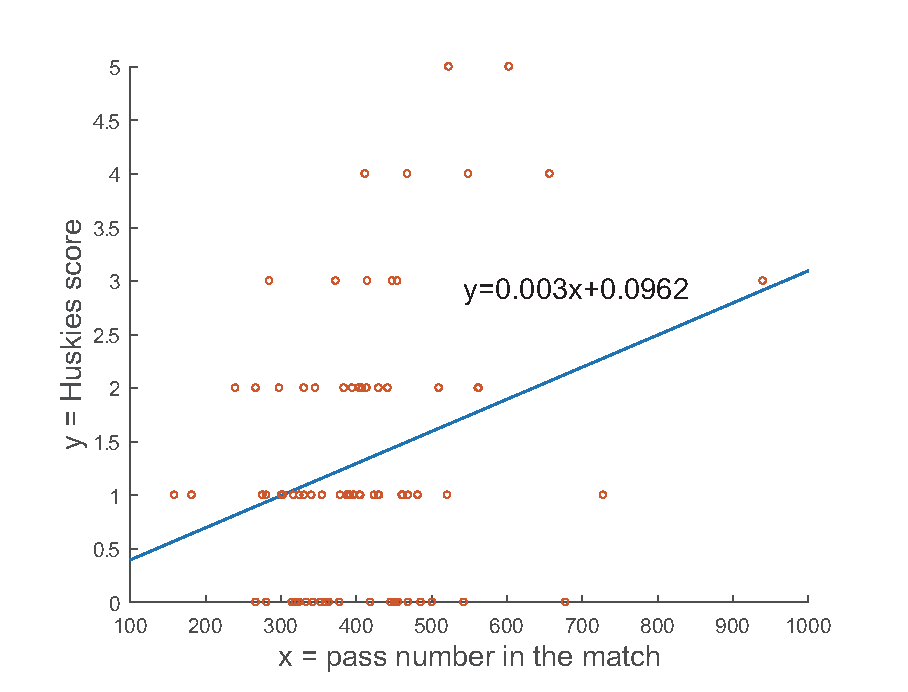
\includegraphics[width=.6\textwidth]{score-pass.eps}
	\caption{The relation between Huskies score and the pass in match.}
	\label{score-pass}
\end{figure}

\subsection{Whole-match Indicator 2: The Total Link Weight}
We surmise that the link weight of the network we obtained above is a more scientific indicator for team cooperation. After all, we take not only the pass number, but also the pass quality (the effect of the passes to subsequent match process) into consideration when calculating the link weight. For simplicity, we only study the sum of the link weight
\begin{equation}
	W=\sum_{m=1}^{11}\sum_{n=1}^{11}W_{m,n}
\end{equation}
in this subsection and leave the spatial and temporal distribution of link weight for later analysis.

To make formula of link weight more scientific, we add a risk contribution, $ax_{m,n,k}$, to the original link weight:
\[
	W_{m,n}=\sum_{k=1}^{K}(B+E_{m,n,k}+S_{m,n,k}+ax_{m,n,k}).
\]
where $x_{m,n,k}$ is the $x$-coordinate of the destination position of the $k$th pass from player $m$ to player $n$ and $a$ is a negative constant, since the more the ball is passed forward, the more the possibility that the ball is lost is. We reset the value of $B$ and adjust the value of $a$ to maximize the correlation between Huskies' score and the total link weight. The final value of $B$ is set to be $1.13$ and the final value of $a$ is $-0.0017$. The correlation between Huskies' score and the total link weight is $0.371$. The fitting formula is
\begin{equation}
	\textbf{Huskies' score}=0.07W+1.3198,
\end{equation}
and the fitting plot is shown in figure \ref{score-W}. Although the correlation is still relatively low, it is higher than that in last subsection, so we regard $W$ as a better indicator for teamwork success.
\begin{figure}[h]
	\centering
	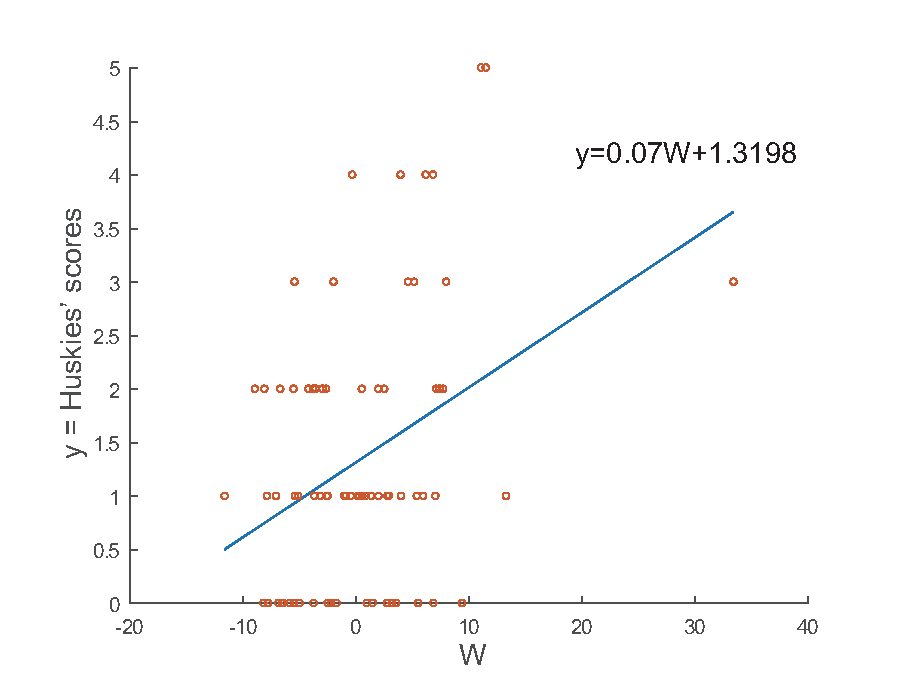
\includegraphics[width=.6\textwidth]{score-W.eps}
	\caption{The relation between Huskies score and the total link weight, $W$.}
	\label{score-W}
\end{figure}

\subsection{The Spatial Distribution of the Indicators}
Besides whole-match indicators of the all players, we investigate into the spatial distribution of Indicators. We attribute different color to the point on the field to present the pass number (figure \ref{FootballFieldPassNumberDistribution}) and the average weight per link (figure \ref{FootballFieldAverageLinkWeigtDistribution}) originated at the point. From the pass number distribution, we find that Huskies tend to pass the ball to the left side of the field. However, according to the average weight per link distribution, the pass at the right side of the field seems to be relatively more effective. Therefore, Huskies may change their attacking strategy from left-style to right-style.
\begin{figure}[h]
	\centering
	\subfigure[The distribution of pass number.]{
	\label{FootballFieldPassNumberDistribution}
	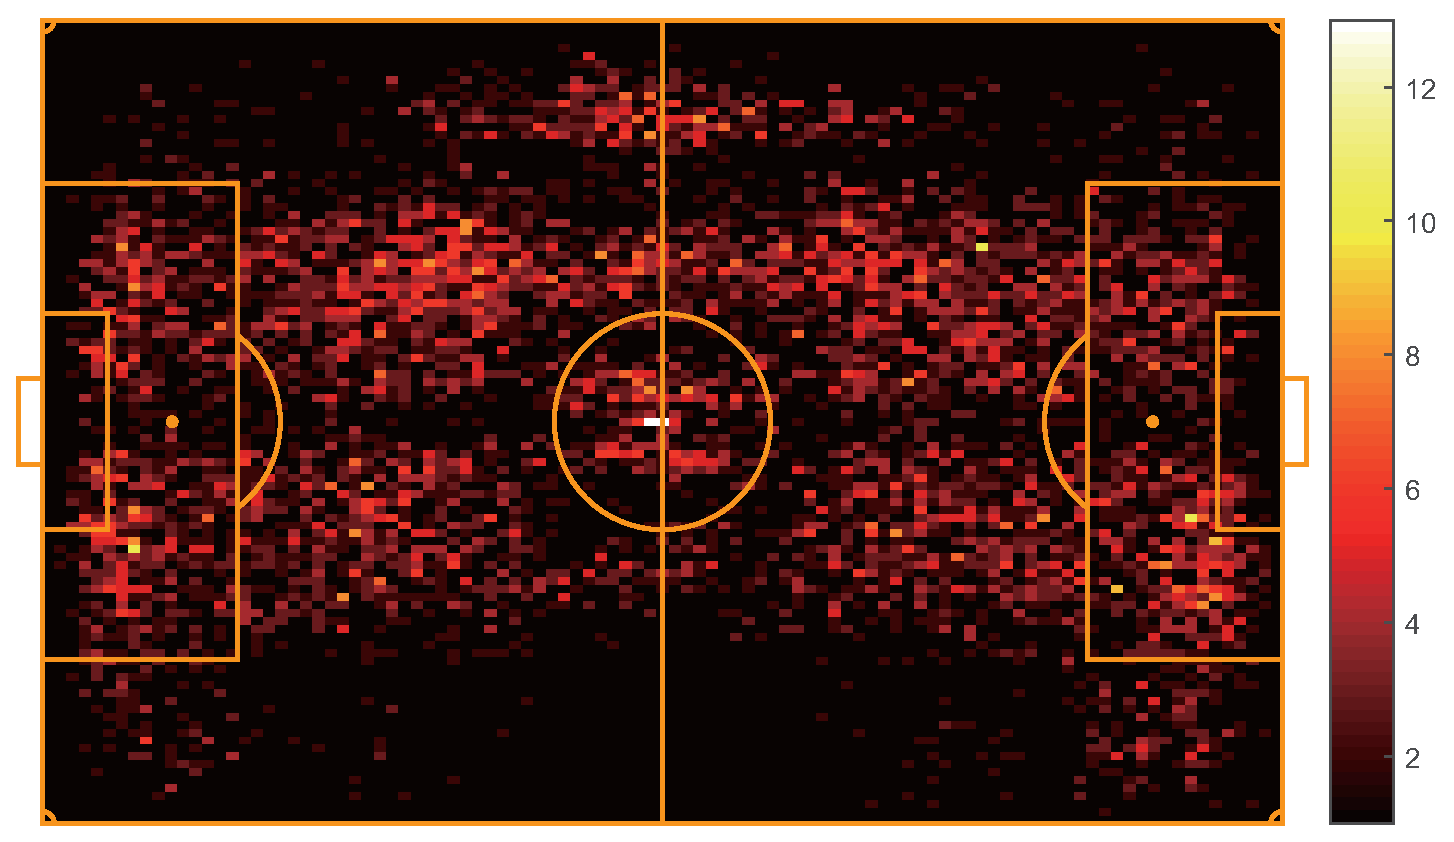
\includegraphics[width=0.45\textwidth]{FootballFieldPassNumberDistribution.eps}}
	\subfigure[The distribution of average weight per pass.]{
	\label{FootballFieldAverageLinkWeigtDistribution}
	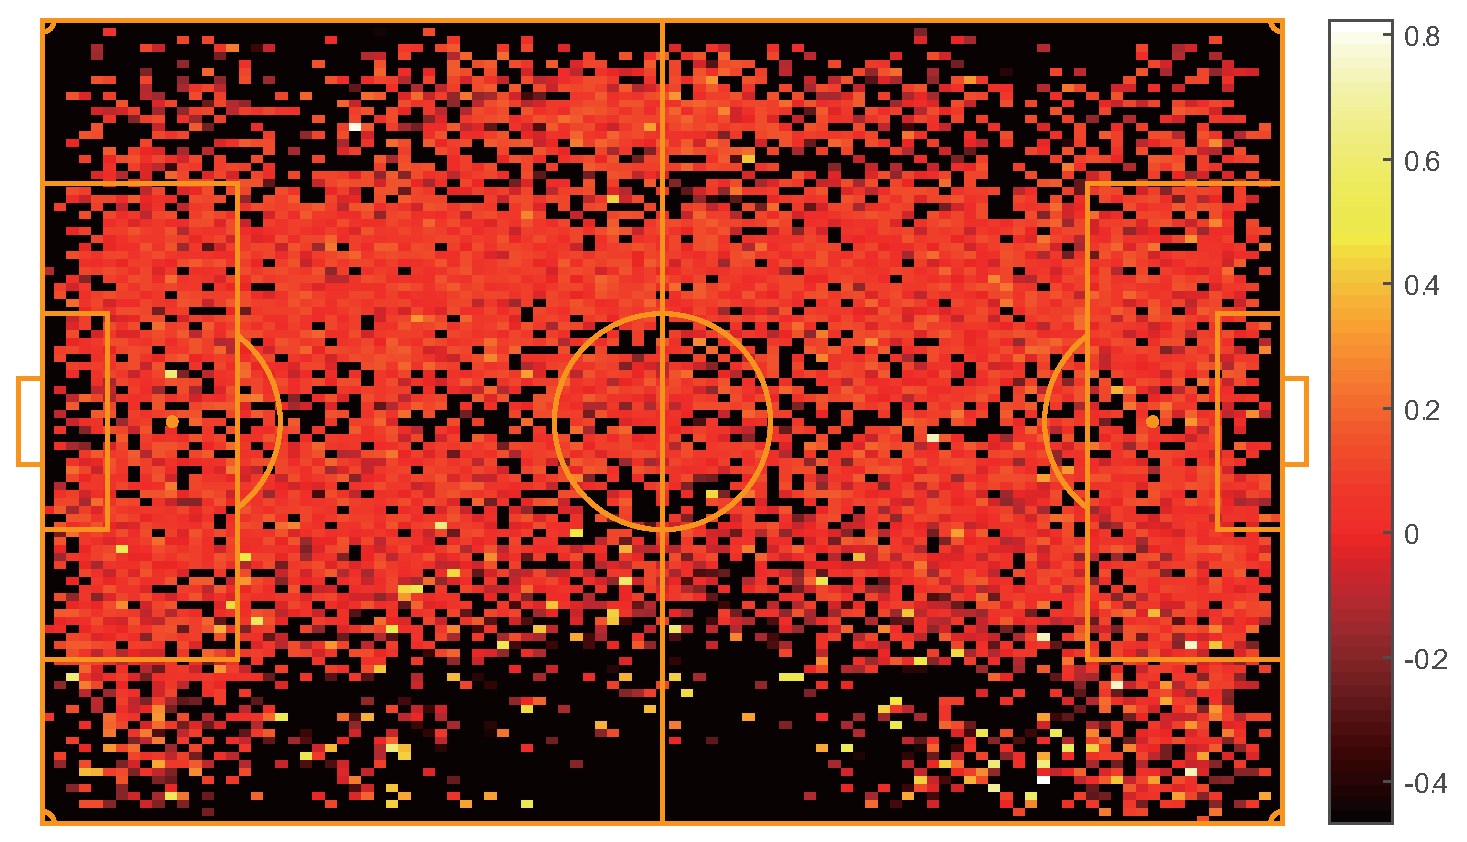
\includegraphics[width=0.45\textwidth]{FootballFieldAverageLinkWeigtDistribution.eps}}
	\caption{The distribution of the two indicators.}
\end{figure}

To eliminate the interference due to the different opponent team, we also plot the distribution of difference of Huskies' and the opponent team's pass number (figure \ref{FootballFieldPassNumberDistribution(ComparedWithCondition)}) and weight per pass (figure \ref{FootballFieldAverageLinkWeightDistribution(CompareWithCondition)}). From the two distribution diagram, we verify the conclusion again. Therefore, our conclusion is universal -- it is solid regardless of the opponent team.
\begin{figure}[h]
	\centering
	\subfigure[The distribution of the difference of pass number of Huskies and the opponent team.]{
	\label{FootballFieldPassNumberDistribution(ComparedWithCondition)}
	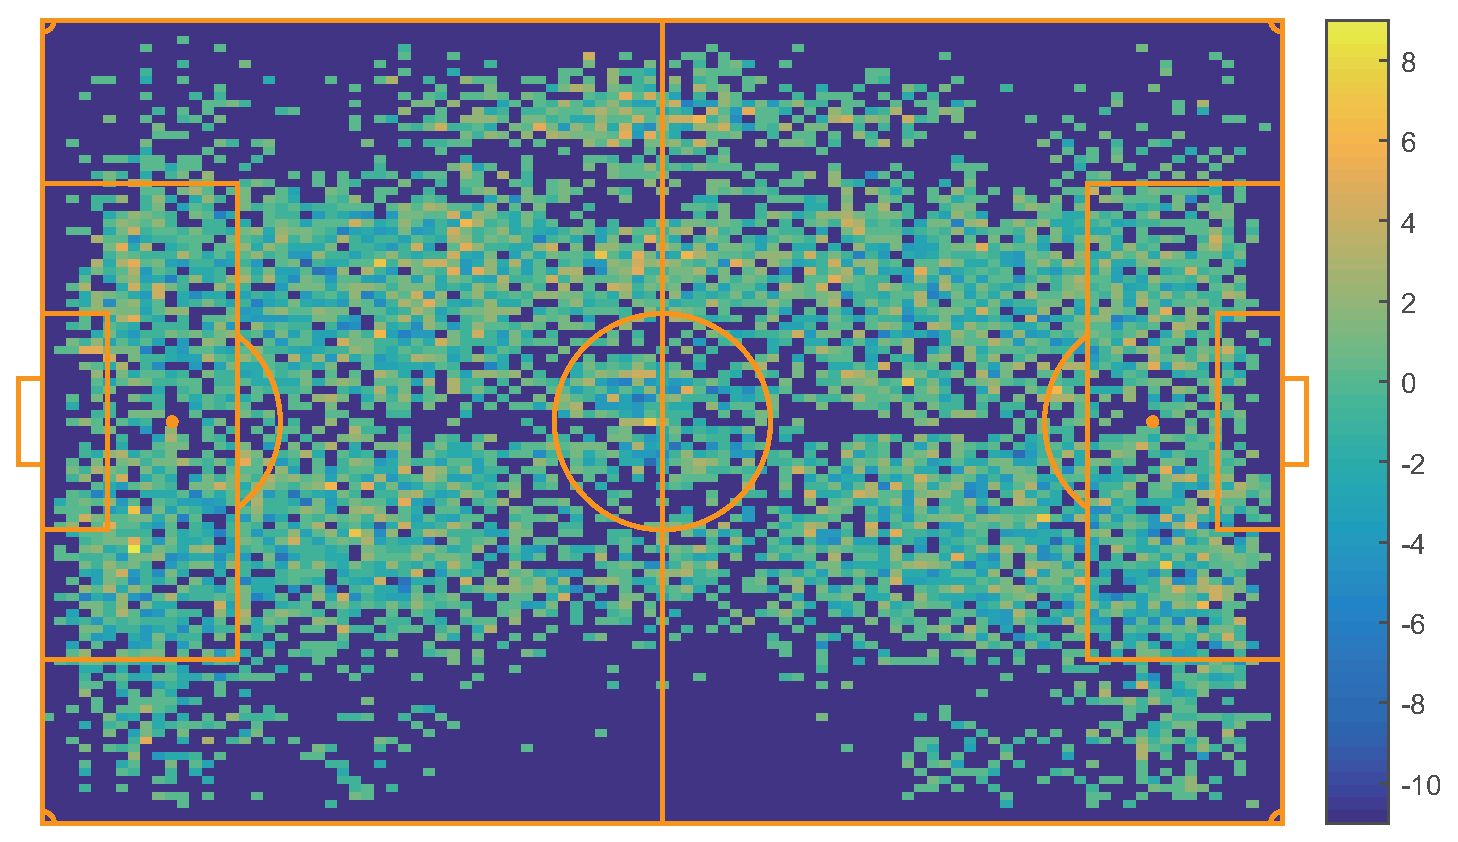
\includegraphics[width=0.45\textwidth]{FootballFieldPassNumberDistribution(ComparedWithCondition).eps}}
	\subfigure[The distribution of the difference of average weight per pass of Huskies and the opponent team.]{
	\label{FootballFieldAverageLinkWeightDistribution(CompareWithCondition)}
	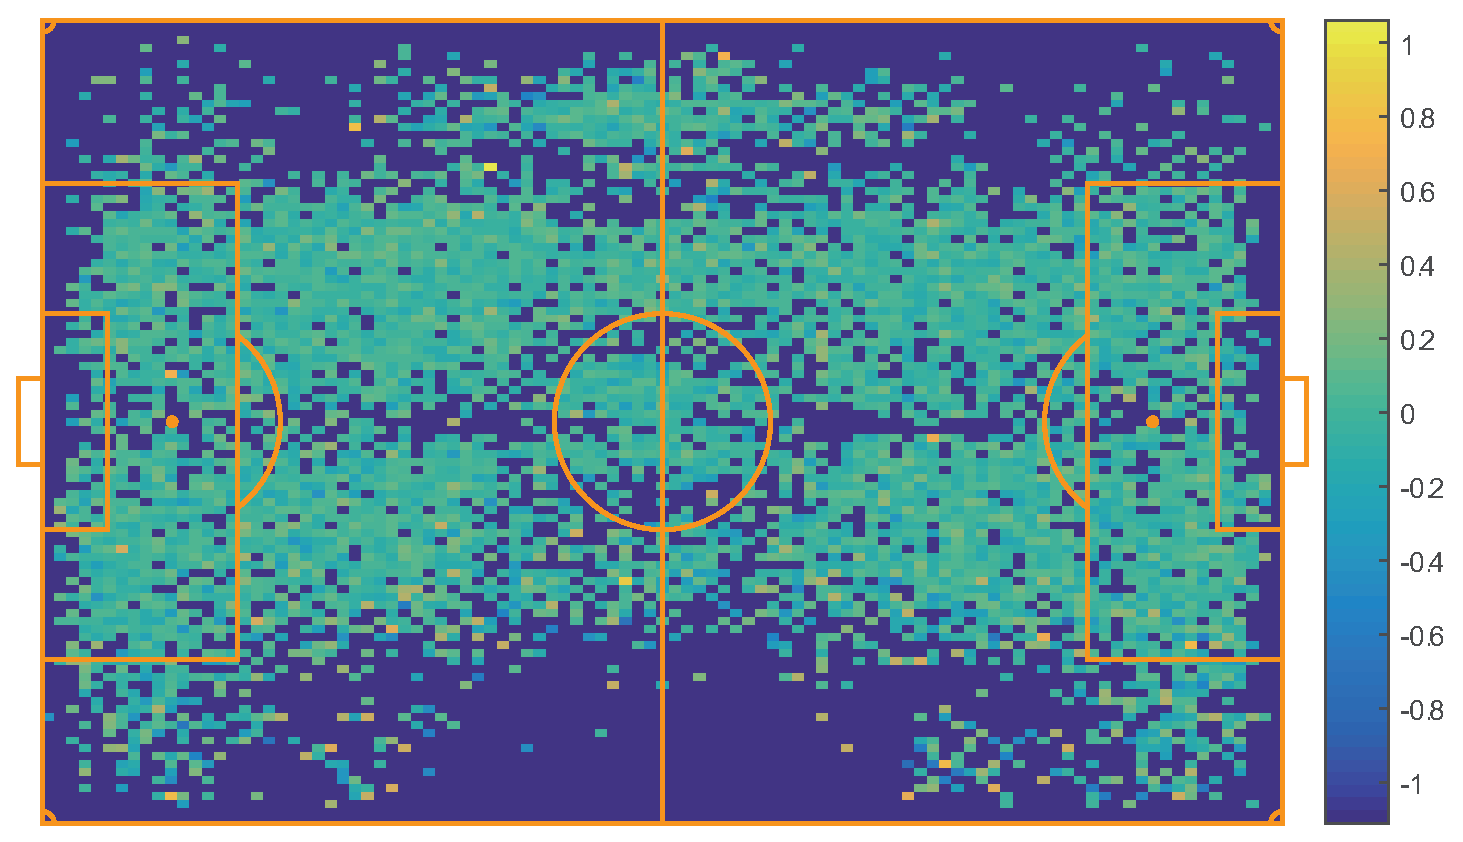
\includegraphics[width=0.45\textwidth]{FootballFieldAverageLinkWeightDistribution(CompareWithCondition).eps}}
	\caption{The distribution of the two indicators.}
\end{figure}

\subsection{Evaluating the Players with the Indicator}
In this subsection, we evaluate the performance and the value of each player with the help of the indicators. First, we show the average weight per pass of the pass originated from each player (figure \ref{PlayerContribution}), which can reflect the relative contribution of each player. According to the histogram, the contribution of the players are order as: $\text{goalkeeper}>\text{defense}>\text{midfield}>\text{forward}$. This may be because the player on the front the team are faced with more pressure from the opponent and higher risks of losing the ball, and thus have more difficulty in making effective effort. Comparing the players of the same types, we find that the passes of forward 2, 6, midfield 7 and defense 1, 2, 4, 9 are more effective while the forward 3, 4, midfield 8, 9, 12, 13 and defense 8, 10 have less contribution in the team cooperation.
\begin{figure}[h]
	\centering
	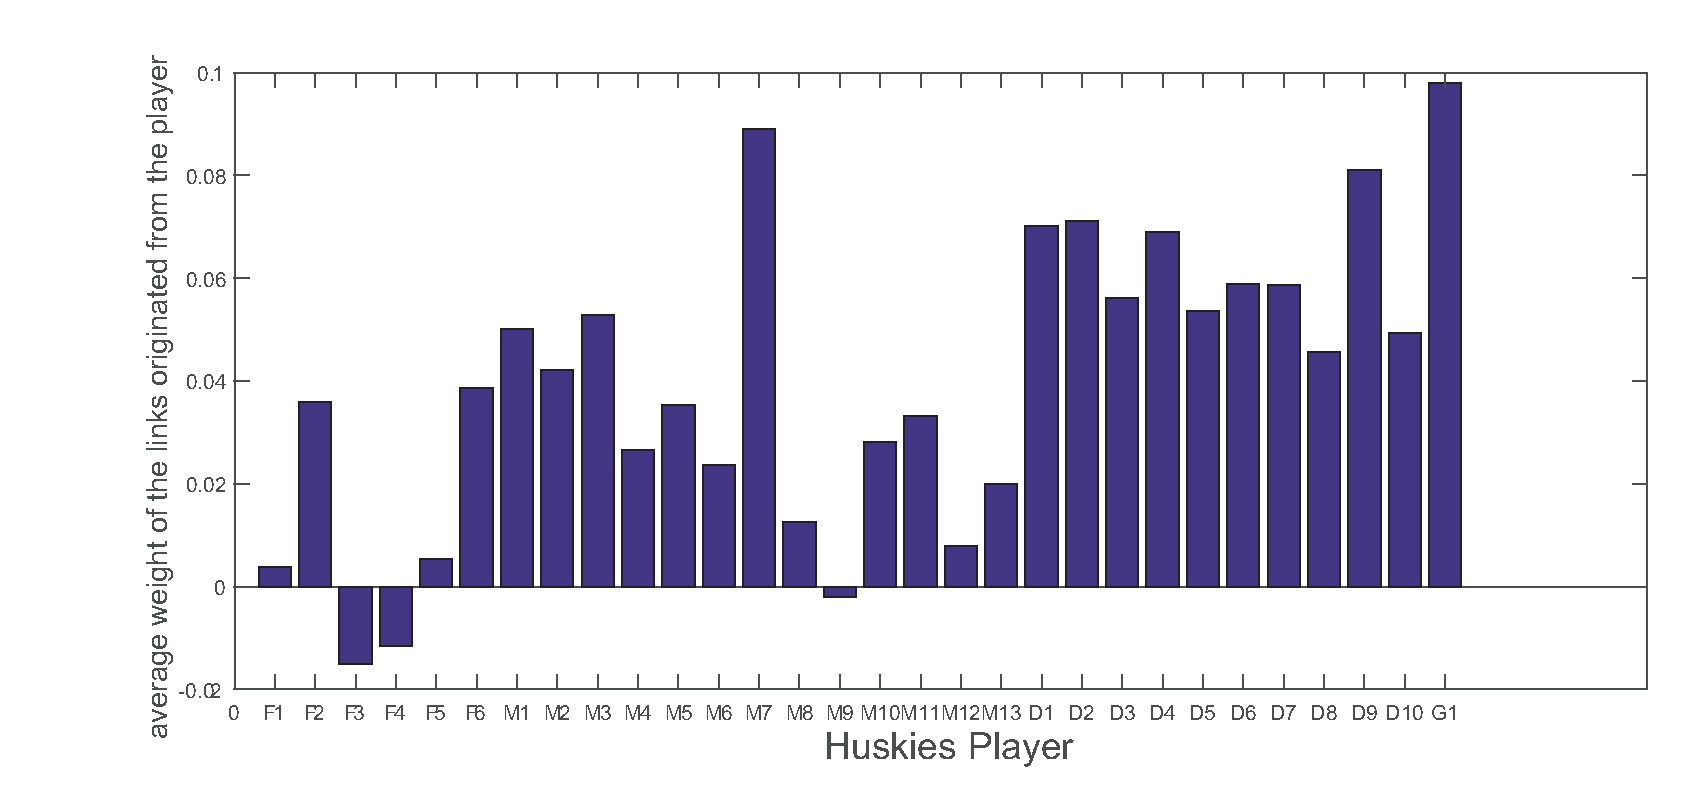
\includegraphics[width=.8\textwidth]{PlayerContribution.eps}
	\caption{The average weight of the link originated from each player.}
	\label{PlayerContribution}
\end{figure}

Then we also analyze the average pass number per match of each player (figure \ref{PlayerPassNumber}). Comparing the players of the same type, the forward 2, midfield 1, 3 and defense 1, 3 offers the most frequent passes.
\begin{figure}[h]
	\centering
	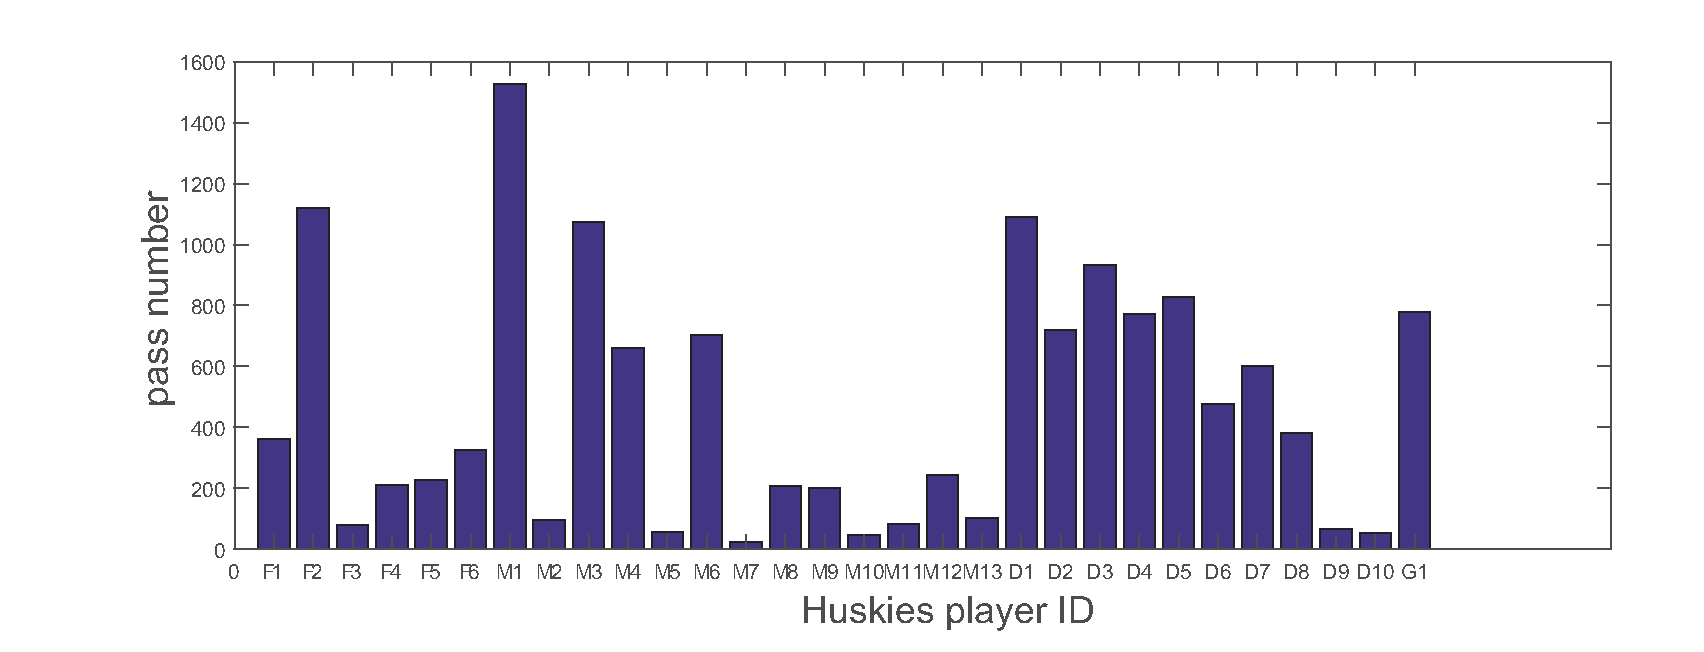
\includegraphics[width=.9\textwidth]{PlayerPassNumber.eps}
	\caption{The average pass number per match of each player.}
	\label{PlayerPassNumber}
\end{figure}

The player combination appeared most frequently in the $38$ matches is
\begin{itemize}
	\item \textbf{Forward:} 1, 2
	\item \textbf{Midfield:} 1, 3, 4, 6
	\item \textbf{Defense:} 1, 3, 4, 5
	\item \textbf{Goalkeeper:} 1
\end{itemize}
However, taking the two indicators into consideration, we recommend such a player combination for best cooperation:
\begin{itemize}
	\item \textbf{Forward:} 2, 6
	\item \textbf{Midfield:} 1, 2, 3, 7
	\item \textbf{Defense:} 1, 3, 4, 9
	\item \textbf{Goalkeeper:} 1
\end{itemize}
Two promising, player midfield 7 and defense 9, need more opportunities.

\section{Temporal Variation of the Indicators}
As the match goes on, the indicators of team success evolve, so we also investigate the temporal distribution of the indicators. We plot the curve of the pass number per minute and the contribution to the total link weight per minute varying with time (figure \ref{variation}). These two curves both present a decline trend at the end of the match. We comprehend the decline as a result of the lack of the strength or the lax attitude of the player before the end of the match. Therefore, the end of a match may be the most dangerous period for Huskies due to less cooperation and it is necessary to give the players more physical training and remind them to remain alert at the end of a match.
\begin{figure}[h]
	\centering
	\subfigure[The variation of pass number of Huskies per minute during a match.]{
	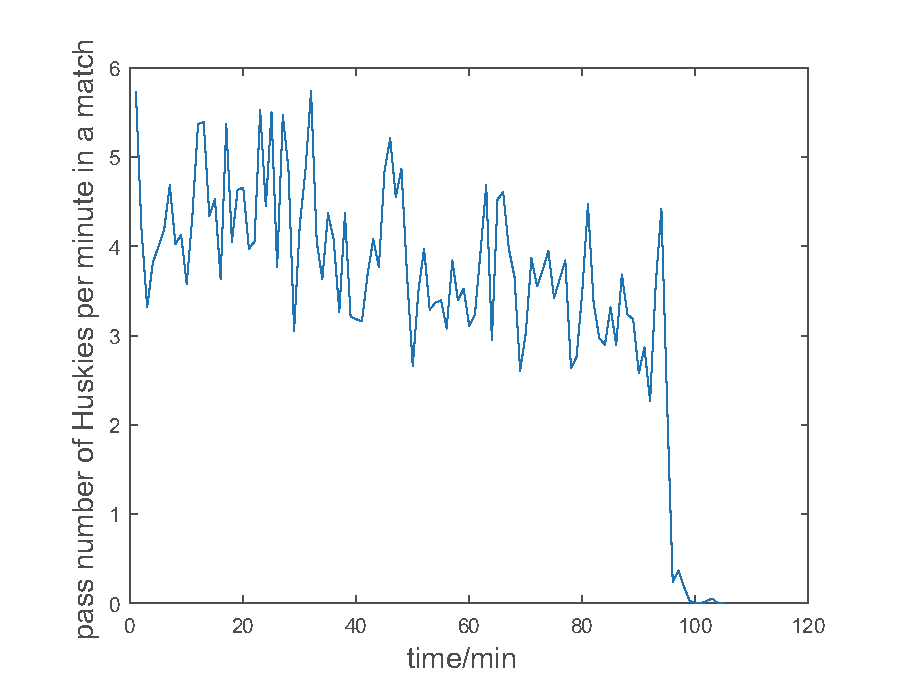
\includegraphics[width=0.45\textwidth]{W-t.eps}}
	\subfigure[The variation of the contribution to the total link weight of Huskies per minute during a match.]{
	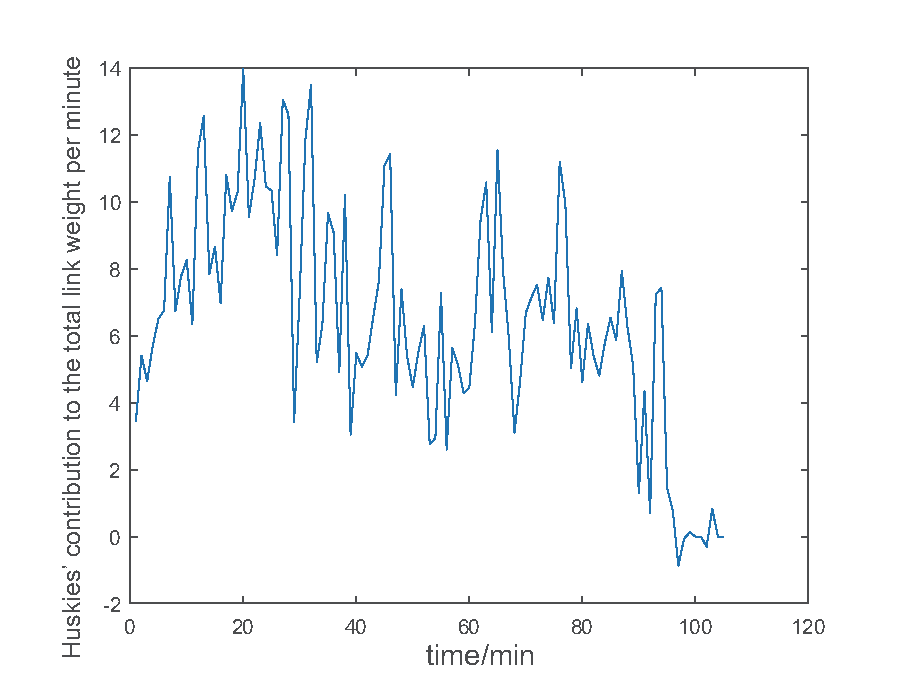
\includegraphics[width=0.45\textwidth]{contribution-t.eps}}
	\caption{The variation of the two indicators during a match.}
	\label{variation}
\end{figure}

\section{Strengths and weaknesses}
\subsection{Strengths}
Here are the strengths of our modeling:
\begin{itemize}
    \item We do not only take the pass as a indicator of the cooperation between the players, but also use the after-pass effect to evaluate the quality of each pass.
    \item Our study of the two indicator covers multiple scales, from the whole Huskies team to every individual player, from the whole matches to the variation per minute.
    \item We introduce the novel concept of threatening degree and ball possessing factor to take the effect of event position on the field and type into consideration.
\end{itemize}

\subsection{Weakness}
Obviously, our modeling also has several weakness:
\begin{itemize}
    \item We omit the event, like foul and save attempt, which may make change to the score of the teams, for simplicity.
    \item The correlation between the indicators and the score is still not high enough to some degree.
    \item We do no find any correlation of cooperation pattern and the score after identification of the motifs.
\end{itemize}

\section{Conclusion}
We construct the pass networks to depict the cooperation relationship in Huskies and find the correlation between the two indicators, pass number and link weight, and Huskies' score. According to the knowledge we learn from the pass network, we provide following suggestions for improving the team performance of Huskies:
\begin{itemize}
	\item Huskies player should make more frequent passes (which means more cooperation) and improve the quality passes (the rate of the good passes) to help score.
	\item The best team combination is forward  2, 6, midfield 1, 2, 3, 7, defense 1, 3, 4, 9, and goalkeeper 1.
	\item The Huskies should change their attacking strategy from left-launched to right-launched.
	\item The Huskies should increase stamina training and keep alert constantly to maintain good cooperation at the end of the match.
\end{itemize}

The analysis of teamwork in football matches gives us universal inspiration. Actually, close cooperation, good combination of teammates and correct work strategies should alsop be successful factor in team work of other field besides football. The methodology of constructing network for team configuration and find indicators from it may also work for researches on the team process in other field.

\addcontentsline{toc}{section}{Reference}
\bibliography{2018506.bib}
\bibliographystyle{unsrt}%{siam}%unsrt按引用先后排序
\end{document}
\end
